\documentclass{article}
\usepackage{MNotes}
\usepackage{amssymb}
\usepackage{bussproofs}
\title{\huge{\textbf{Assignment 3}}}
\author{\Chi{杨乐天}}
\date{}

\newcommand \ran[1]							{\text{Ran}\left( #1 \right)}
\newcommand \logequiv						{\vDash\mathrel{\text{\reflectbox{$\vDash$}}}}

\begin{document}
\maketitle

\section*{Problem 1}

	The induction hypothesis is stated as follows: for any $\Sigma, \alpha$ satisfying $\Sigma \vdash \alpha$ within height $h-1$, we know that $\Sigma \vDash \alpha$.
	
	Given the induction hypothesis, we work on the case when height is $h$.

\subsection*{(a)}

	Assume we prove $\Sigma \vdash \beta$ through $\perp$-introduction, let $\beta=\alpha\to\perp$, then we know that $\Sigma; \alpha \vdash \perp$ within height $h-1$. By induction hypothesis, for any truth assignment $v$, if $\forall \gamma \in \Sigma; \alpha$, $\bar{v} (\gamma)=T$, then $\bar{v} (\perp)=T$. However, $\bar{v}'(\perp)=F$ for any assingment $v'$. Therefore, $\Sigma; \alpha$ is unsatisfiable, which means any assignment $v$ satisfying all elements in $\Sigma$ has $\bar{v}(\alpha)=F$, and thus $\bar{v}(\alpha\to\perp)=\bar{v}(\alpha)\to\bar{v}(\perp)=F\to F=T$.
	
	%Therefore, for assignment $v$ satisfying $\forall \gamma \in \Sigma$, $\bar{v}(\gamma)=T$, if $\bar{v}(\alpha)=T$, then by the result given above, $\bar{v}(\perp)=T$. Therefore, $\bar{v}(\alpha\to\perp)=\bar{v}(\alpha)\to \bar{v}(\perp)=T\to T = T$. But if $\bar{v}(\alpha)=F$, then $\bar{v}(\alpha\to\perp)=T$ whatever the truth value of $\perp$. Consequently, we have concluded that $\bar{v}(\alpha\to\perp)=T$, that is $\Sigma \vDash \alpha\to\perp$.
	
\subsection*{(b)}

	Assume we prove $\Sigma \vdash \alpha$ through $\perp$-elimination, then $\Sigma \vdash \perp$ within height $h-1$. Similarly, we know from $\Sigma \vDash \perp$ that $\Sigma$ is unsatisfiable, which naturally leads to $\Sigma \vDash \alpha$.
	


\section*{Problem 2}

\subsection*{(a)}

	With complexity seen in directly proving this wff, we prove it through the completeness of sentential logic. For any truth assignment $v$, $\bar{v}(A\to B)=F$ iff. $v(A)=T$ and $v(B)=F$. Therefore, if $v(A)=T$ and $v(B)=F$, $\bar{v}(A\land \neg B)=v(A) \land \neg v(B)=T$; otherwise, $\bar{v}(A\to B)=T$. Consequently, $\bar{v}((A\to B)\lor (A\land \neg b))=T$. Then by completeness of sentential logic, this wff is provable.
	
\subsection*{(b)}

	Let $v(A)=T$ and $v(B)=F$, then $\bar{v}((A\to B)\lor (A \land B))=\bar{v}(A\to B) \lor \bar{v}(A\land B)= F \lor F = F$. Similarly, by the completeness of sentential logic, this wff is not provable.
	
	

\section*{Problem 3}

	In $\forall y (Pxy \to \forall x Pxy)$, the first $x$ occurs free.
	
	In $\forall x (Q y \to \exists y Pxz)$, $z$ and the first $y$ occurs free.
	
	In $(\neg \exists y R(fyz)) \land (\forall x \forall y R(fyz))$, the only free-occurring variable is $z$.




\section*{Problem 4}

	Let $Pxy$ denotes $x$ shaves $y$. Then the problem is to derive $\neg \exists x \forall y (Pxy \leftrightarrow \neg Pyy)$.
\begin{figure}[htbp]
	\centering
	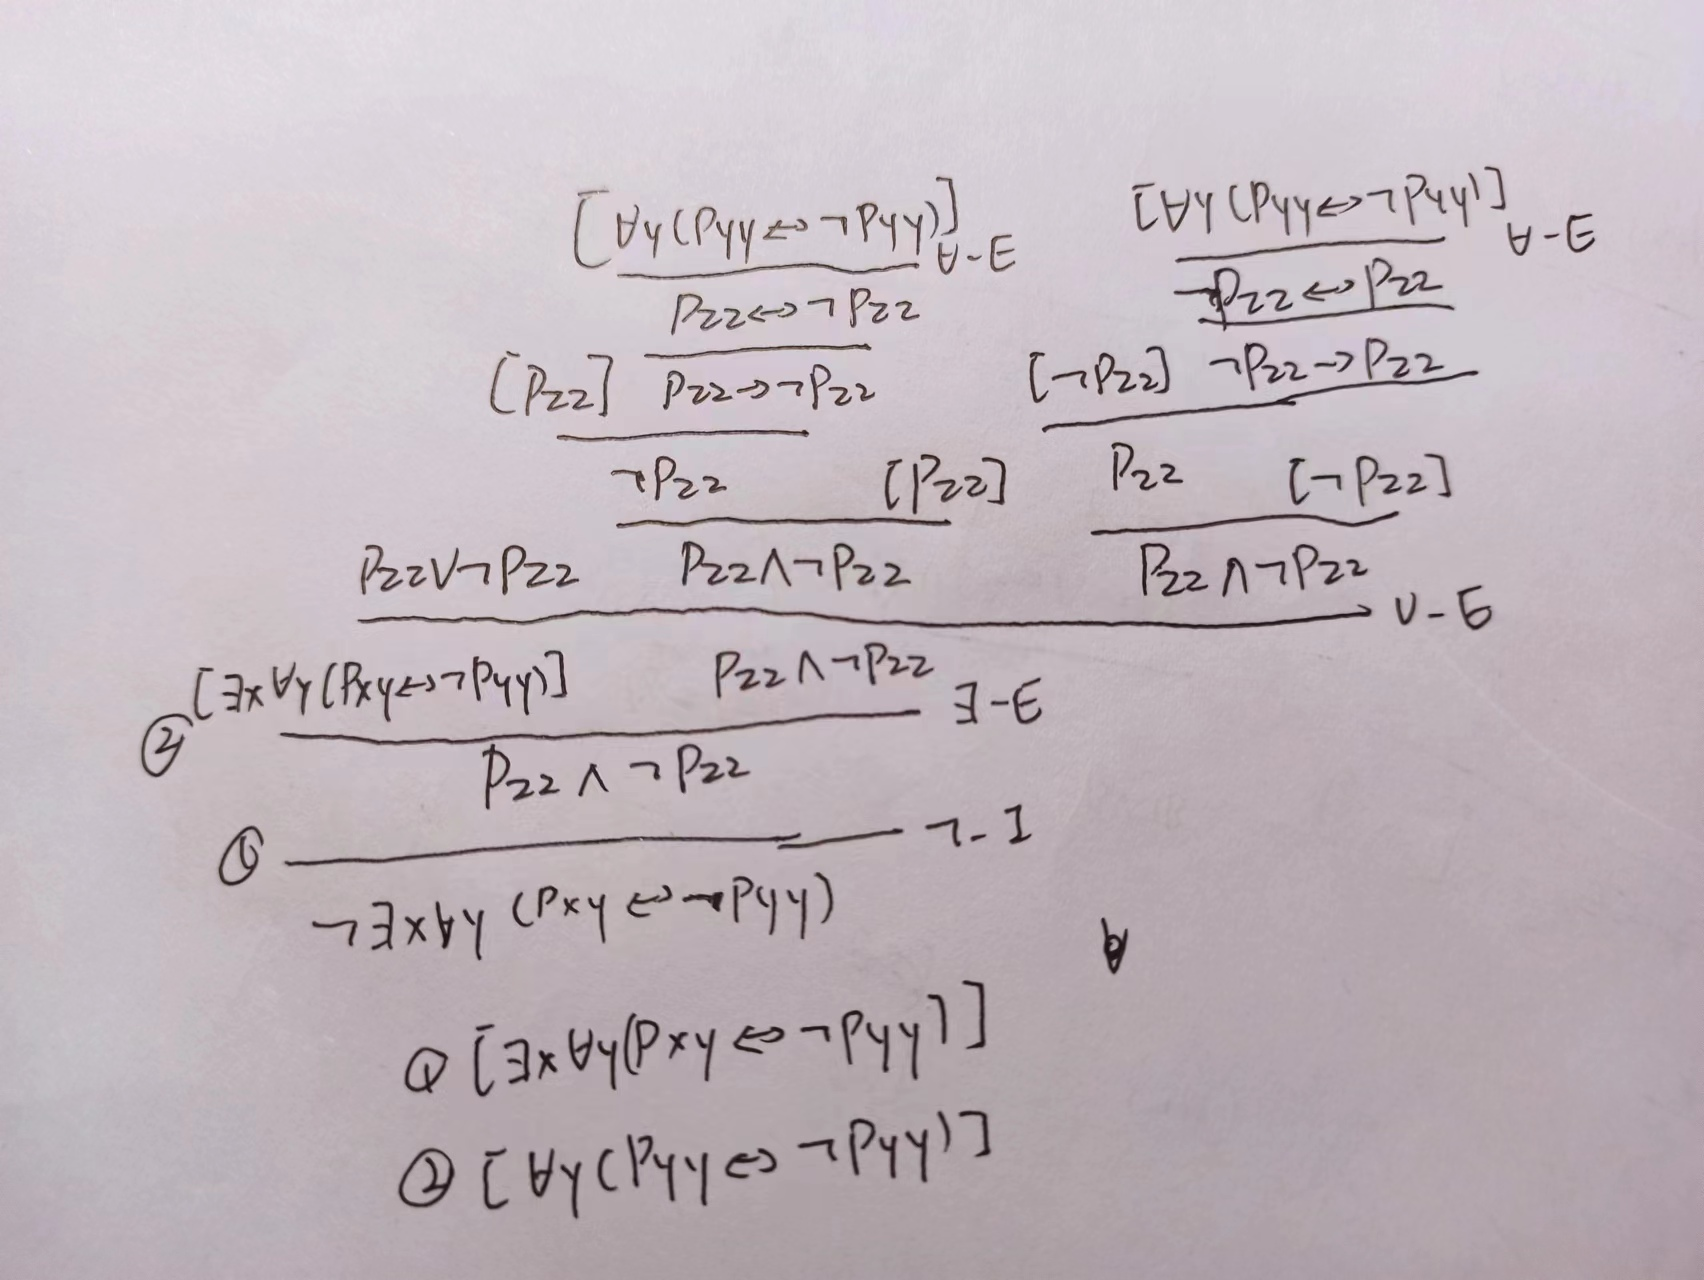
\includegraphics[width=7cm]{prob4.jpg}
\end{figure}



\section*{Problem 5}

\subsection*{(a)}

\begin{figure}[htbp]
	\centering
	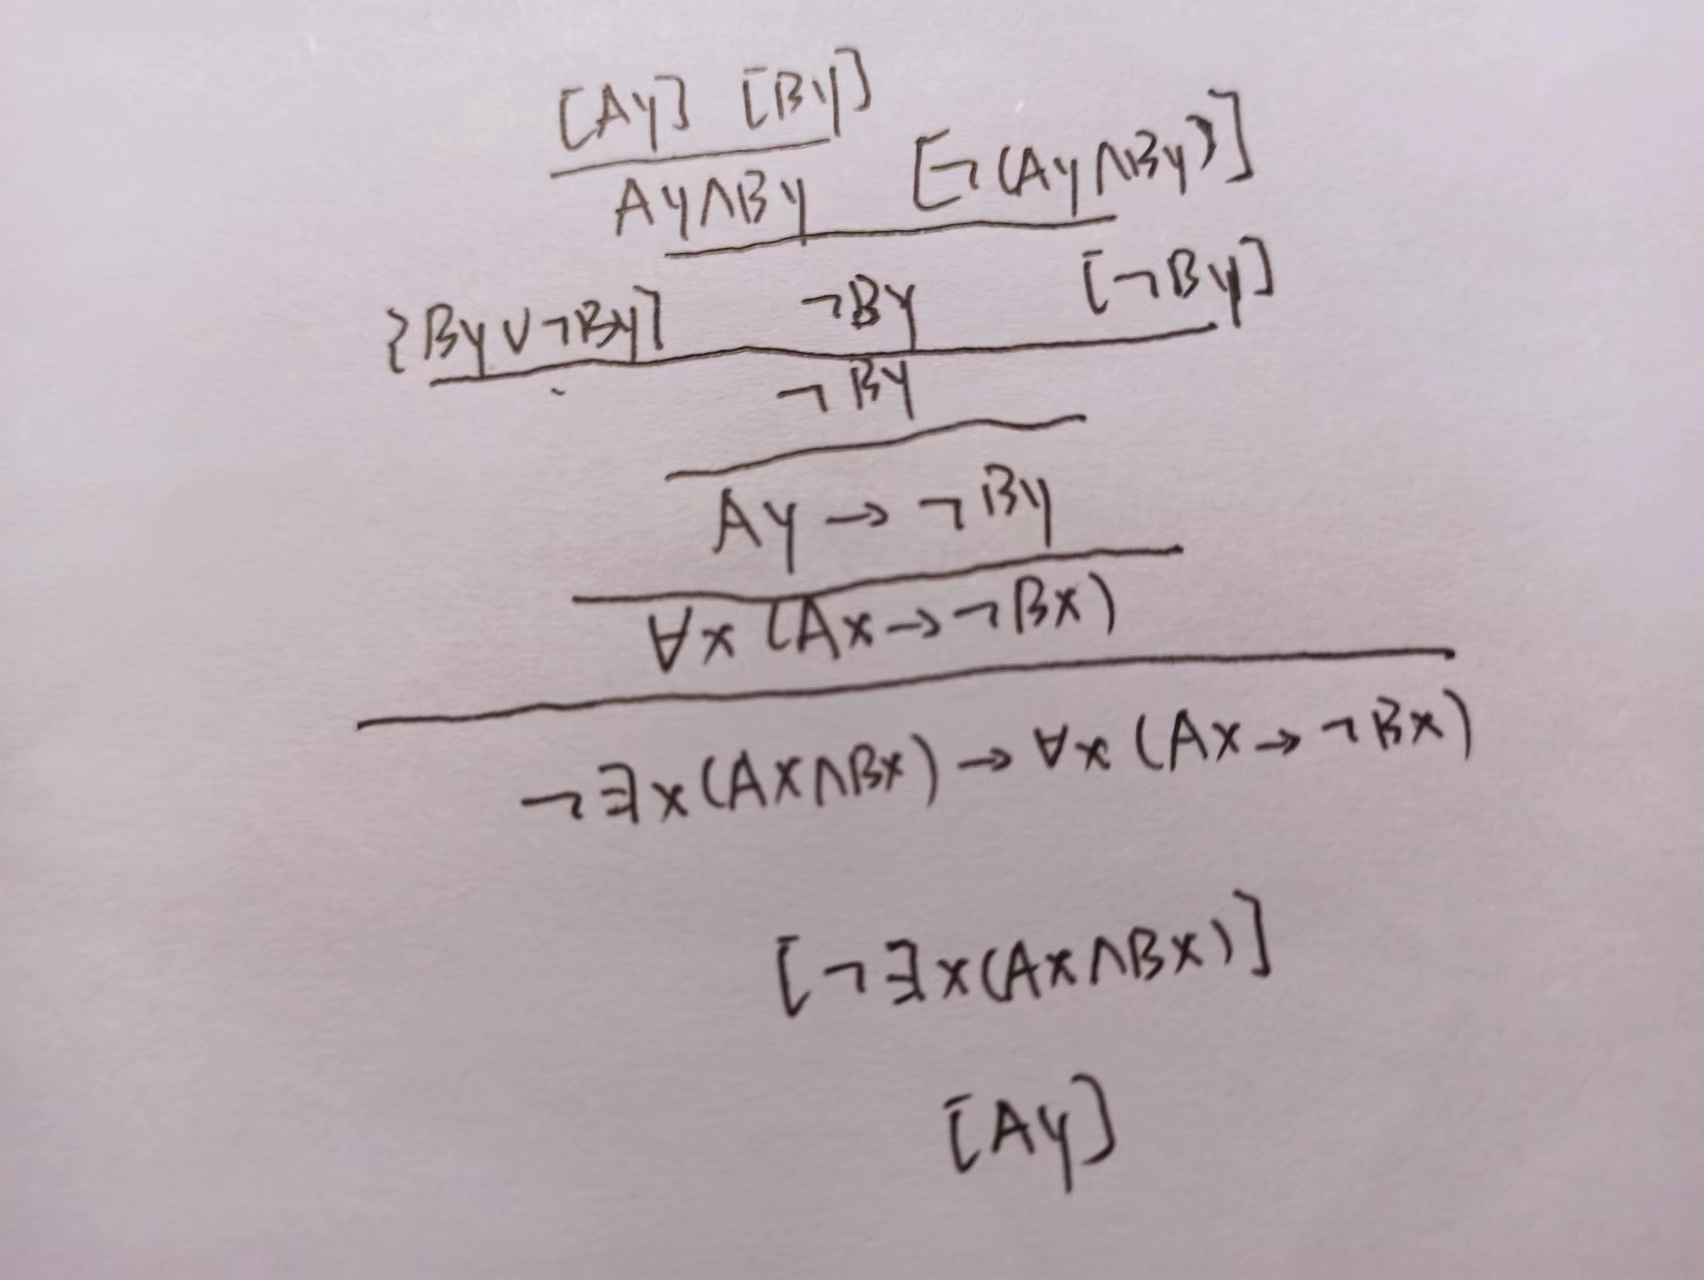
\includegraphics[width=7cm]{prob5a.jpg}
\end{figure}

\subsection*{(b)}

\begin{figure}[htbp]
	\centering
	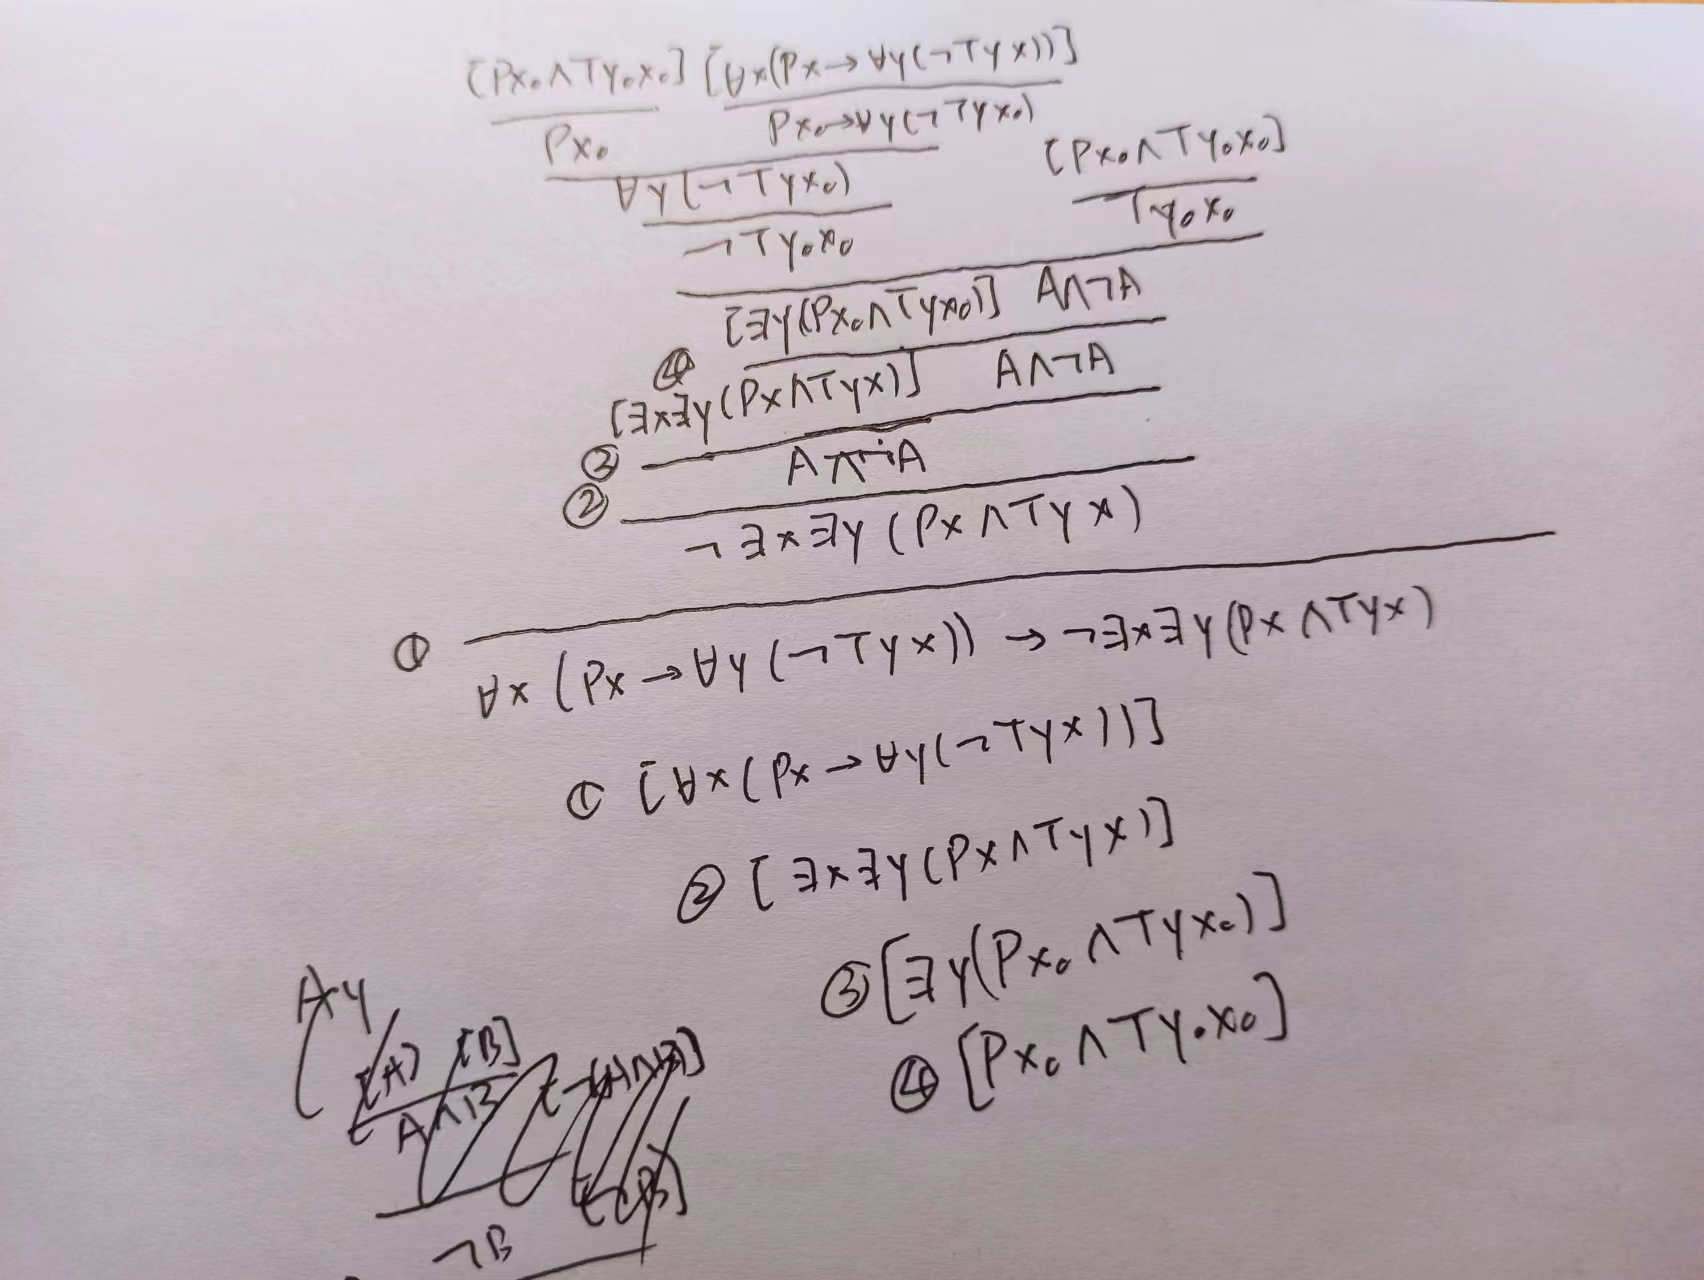
\includegraphics[width=9cm]{prob5b.jpg}
\end{figure}



\section*{Problem 6}

The four statements are (1) $\forall x (Yx \land Hx \to Bx)$, (2) $\forall x (Ax \to Hx)$, (3) $\exists x (Yx \land Ax)$, (4) $\exists x Bx$.

\begin{figure}[htbp]
	\centering
	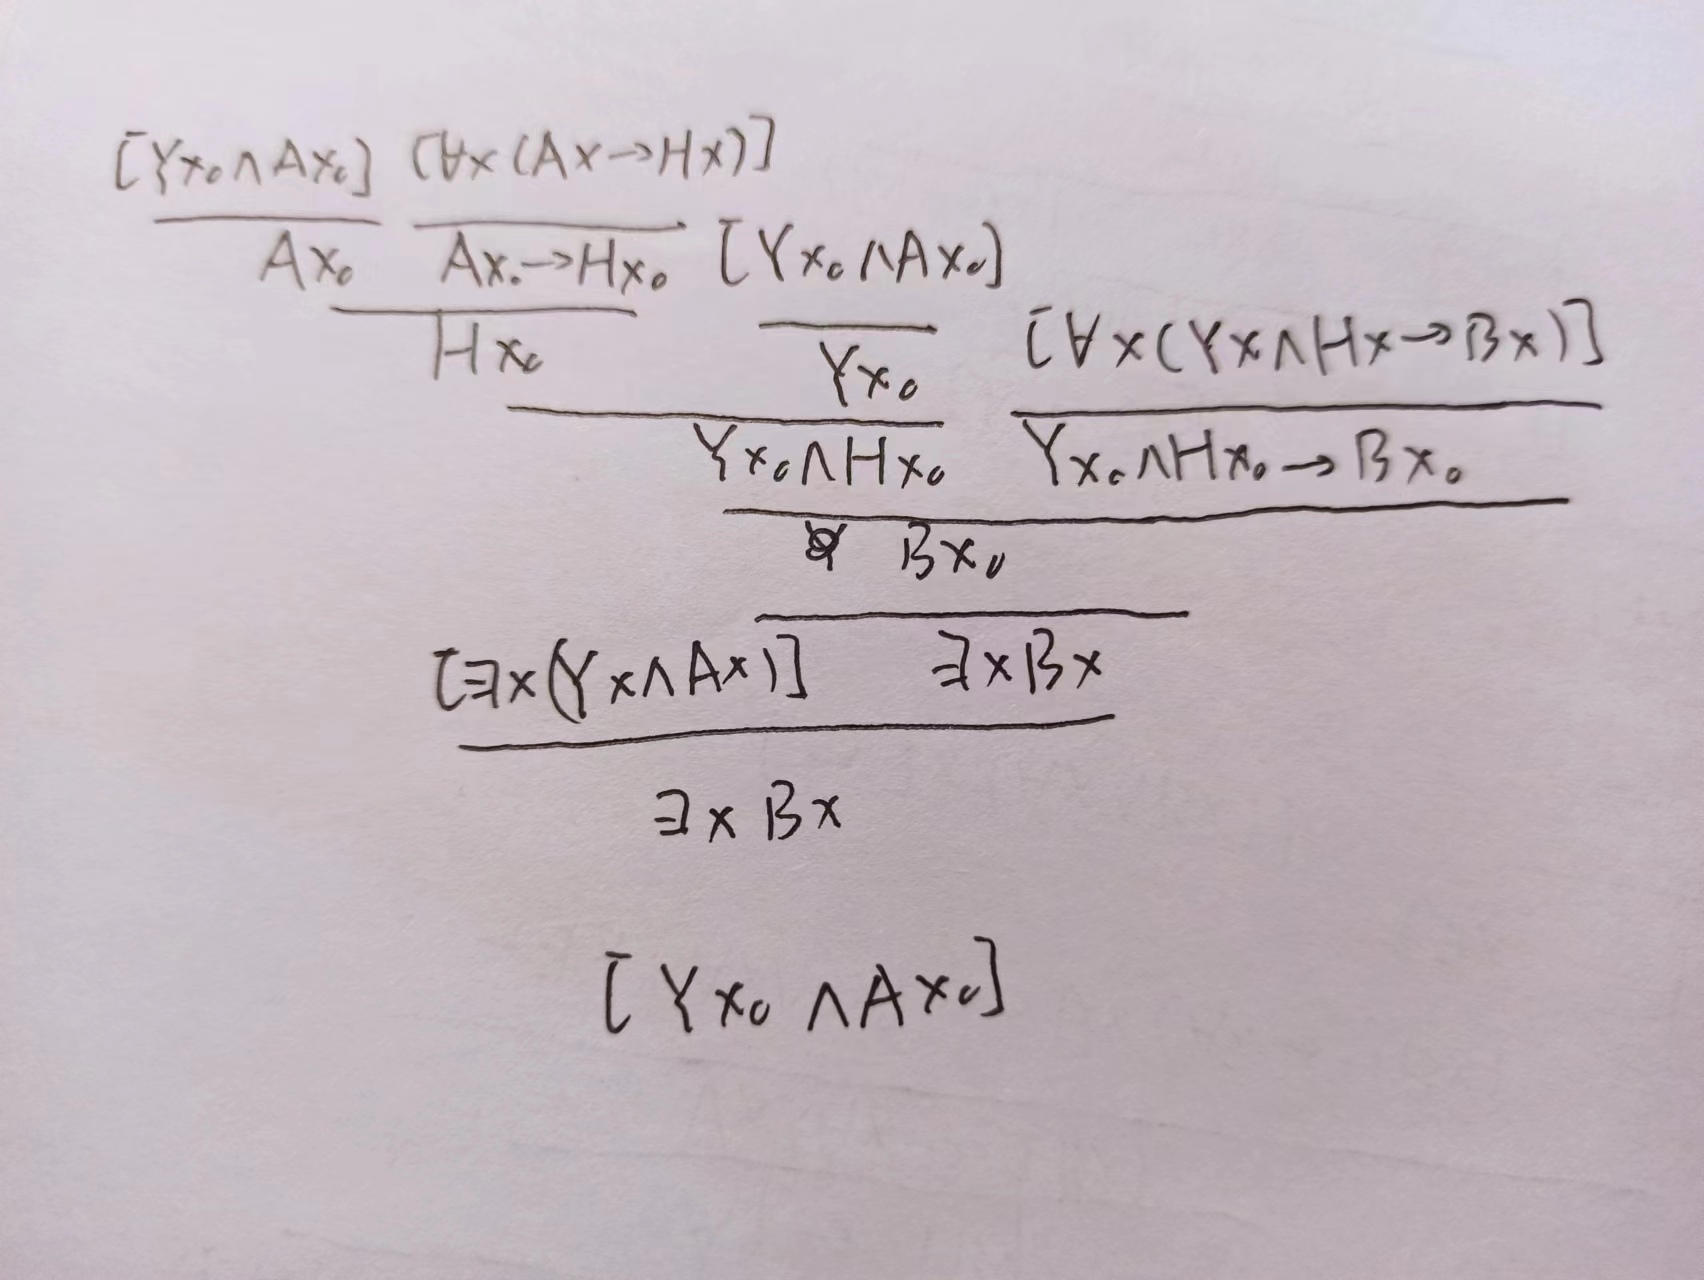
\includegraphics[width=10cm]{prob6.jpg}
\end{figure}



\end{document}